\documentclass[a4paper]{article}

%% Language and font encodings
\usepackage[english]{babel}
\usepackage[utf8x]{inputenc}
\usepackage[T1]{fontenc}

%% Sets page size and margins
\usepackage[a4paper,top=3cm,bottom=2cm,left=3cm,right=3cm,marginparwidth=1.75cm]{geometry}

%% Useful packages
\usepackage{amsmath}
\usepackage{graphicx}
\usepackage[colorinlistoftodos]{todonotes}
\usepackage[colorlinks=true, allcolors=blue]{hyperref}
\usepackage{caption}
\usepackage{subcaption}
\usepackage{float}

%% matlab
\usepackage[framed,numbered,autolinebreaks,useliterate]{mcode}
\usepackage{verbatim}

\title{ECE49600 Undergrad Research Semester Report \\
  \large Photon counting for super-resolution imaging \\
  \large Spring 2022, 3 credit hours.  }

\author{Michael Langford \newline \\
        Instructor: Dr. Kevin Webb}

\begin{document}

\maketitle

\begin{abstract}
During the course of the semester, I worked to prepare for super resolution imaging lab experiments using photon counting apparatus via lab work conducting initial tests, and analyzing the resulting data. In addition to the experimental work I reviewed literature relating to photon counting and work with potential application to photon counting / super-resolution experiments planned for our group.

I was able to assist in conducting multiple tests of the photon counting equipment, with the goal validating its operation and characterizing its behaviour. The goal is to use this device in more complex setups for super-resolution imaging experiments. The equipment is newly acquired however, so it is first necessary to become acquainted with it and ensure it is operating within the advertised parameters. 
The tests primarily consist of using the photon counting equipment to measure the pulse shape of a pulsed laser and working to ensure the measured pulse matches, as closely as possible through iteration of experiments, the proscribed pulse shape from the pulsed laser.

This device should be very useful in the future for multiple experiments where time-correlation of laser signals are desired, as this device is very helpful for collecting this information. In particular, we are interested in using photon counting devices to create a Hanburry Brown-Twiss Interferometer to access higher order correlation information. 
In the characterization of the hardware, multiple setups were used as issues were debugged and solutions found. I present the details of each setup as well as an analysis of the results of the experiments for each setup, and recommendations to improve the performance of the equipment for future usage in more complex experiments.

In reviewing published material, I read multiple papers with relevance to photon counting and super-resolution imaging, and learned about the various ways that super-resolution imaging is being done, and particularly how photon-counting is applicable to it. I detail what I learned from each paper and a high level overview of it, with an explanation of why it is of particular interest and how it might be useful to the group. 
In particular, I did a more in depth analysis of the math and algorithm described in a paper written on higher order correlations with relevance to photon counting, as the algorithm can be used on the output gathered from a Hanburry Brown-Twiss Interferometer, which may use be implemented via photon-counting. I worked to understand better the implications of the algorithm they describe, and the math of higher order correlations.

\end{abstract}

\section{Lab work}

\subsection{Introduction}

My lab work this semester focused on testing the photon counting equipment to prepare for super-resolution experiments where photon-counting data is required. Thus my work consists of a set of tests of the photon counting equipment as we gained more understanding of the device's operation and fixed issues contributing to error in the photon counting measurement.

The exact goal of this set of experiments is to direct a pulsed laser beam into the SPAD aperture, measure the resulting pulse waveform using the photon counting equipment, and then analyze the data and determine how closely the measured pulse matches the proscribed pulse shape of the pulsed laser waveform. The closer this measurement to the real pulsed laser waveform, the more accurate we can say the photon counting equipment is. Therefore with each setup the goal is to remove possible sources of noise, error, distortion, etc. to determine just how to accurately measure a pulse waveform so that future measurements can be as accurate to the true waveforms as possible.

The photon counting equipment itself consists of a main control box that interfaces to a laptop, and the sensor, which is a SPAD (Single Photon Avalanche Diode) detector mounted within a containing aperture and additional integrated supporting electronics. The photon counting control box connects to the SPAD detector and a laptop, as well as a sync pulse cable coming from the pulsed laser source. This sync pulse allows the photon counting equipment to synchronize its measurements in time to the beginning of a laser pulse.

In addition to the photon counting devices the experiments utilized multiple lasers and their associated devices, along with typical optical table items such as mirrors, filters, lenses, etc.

\subsection{SPAD}

An introduction to the SPAD device itself is in order to understand the reasons guiding the setup and parameters used in each experiment.

At high rate of acquisition and at an invariant interval, the photon counting setup measures the time required for the SPAD to detect the arrival of a single photon. Once it has arrived, the SPAD undergoes complex electrical changes and it is not ready for another detection until the next acquisition interval, though this happens quickly. By plotting a histogram of number of photons that have arrived within a certain time step vs. time, and measuring an optical signal repeatedly (one that can be repeated with an extremely high degree of similarity, e.g. a periodic laser pulse), one can recover the intensity vs. time properties of the signal, and in our application, the pulse shape of the laser pulse incident upon the detector.

There are peculiarities to this method of extracting the pulse shape that are important to remember. Vital is the observation that the SPAD takes advantage of the quantum properties of light, and so either detects one photon, or none for a given instant in time, and once one is detected, it cannot detect again until the next repetition of the signal. Clearly then, the signal must not be so powerful that the probability of a photon arriving from the start of the pulse is high enough to prevent a photon from the tail end of the pulse from being the first to arrive at the detector (all prior photons being either attenuated or having never been transmitted due to their probabilistic nature).

Because the attenuation is time invariant, there is equal probability of photons being attenuated at any point within the laser pulse. With the attenuation low enough such that only one photon or none usually arrive within a single pulse, there will be negligible distortion of the pulse shape from early-arriving photons ‘shadowing’ the tail of the pulse. With the attenuation set properly (in most applications the recommended probability of arrival at all over the entire sensing period is 0.05 or less), the SPAD setup can repeatedly measure photon arrival times, bin them, and create a histogram that accurately represents the waveform of the laser pulse in question.

In addition to the proper attenuation of the laser signal, the timing of the signal is critical. In order to correctly timestamp a photon arrival relative to the beginning of the laser pulse, the photon counting hardware is connected to the laser source via a 'sync pulse' line, an electrical cable that sends out inverted electrical pulses that signal the beginning of a laser pulse.

Timing error in this sync line from the laser source, or phase noise / jitter, can be the cause of a spread in the pulse shape that can appear as if caused by a physical source. Random variation over time of this timing results in incorrect binning of photon arrival times, and the signal becomes spread out / smeared across time. Because the photon counter uses the sync pulse as its temporal reference point, it bins each photon arrival relative to that timestamp, so a random variation in the discrepancy between the sync pulse and the laser signal results in improper binning that differs from the correct time position by a different amount each pulse, which over the course of a measurement results in temporal dispersion of the pulse shape.

\subsection{Initial Setup}
The initial setup used at the beginning of the photon counting experiments consisted of a standalone 635nm Horiba laser diode aimed through a collimating lens, mirrors, and an ND filter, and then into the aperture of the photon counter SPAD. The timing and laser supply controls were kept off to the side together for ease of control.

Initially efforts were focused on getting the photon counter to properly record and bin the photon arrivals at the correct timescale relevant to the expected pulse width, and ensuring the the probability of arrival of a photon at the SPAD aperture was below the recommended threshold. Once this was completed however, it was noticed that the measurement of the pulse width was significantly higher than expected, by orders of magnitude.

Fig.\ref{fig:pulse_1} shows the distorted pulse shape with a decaying tail, much different from the expected symmetrical pulse shape.

Efforts to combat this were based off the idea that photons could be bouncing off items in the setup and resulting temporal dispersion, as some photons would randomly take much longer to arrive. If this effect was independent of the point in the pulse the photon was from, this simply yields the new pulse width as being the convolution of the possible arrival delay range due to the bounces, and the original pulse. This is essentially the temporal point spread function of the device.

The other possible cause of the spread in the pulse shape is the presence of phase noise in the sync line coming into the photon counter from the laser source. Any issues in the precision of this timing results in incorrect binning of photon arrival times, and the signal becomes spread out / smeared across time.

\begin{figure}
\centering
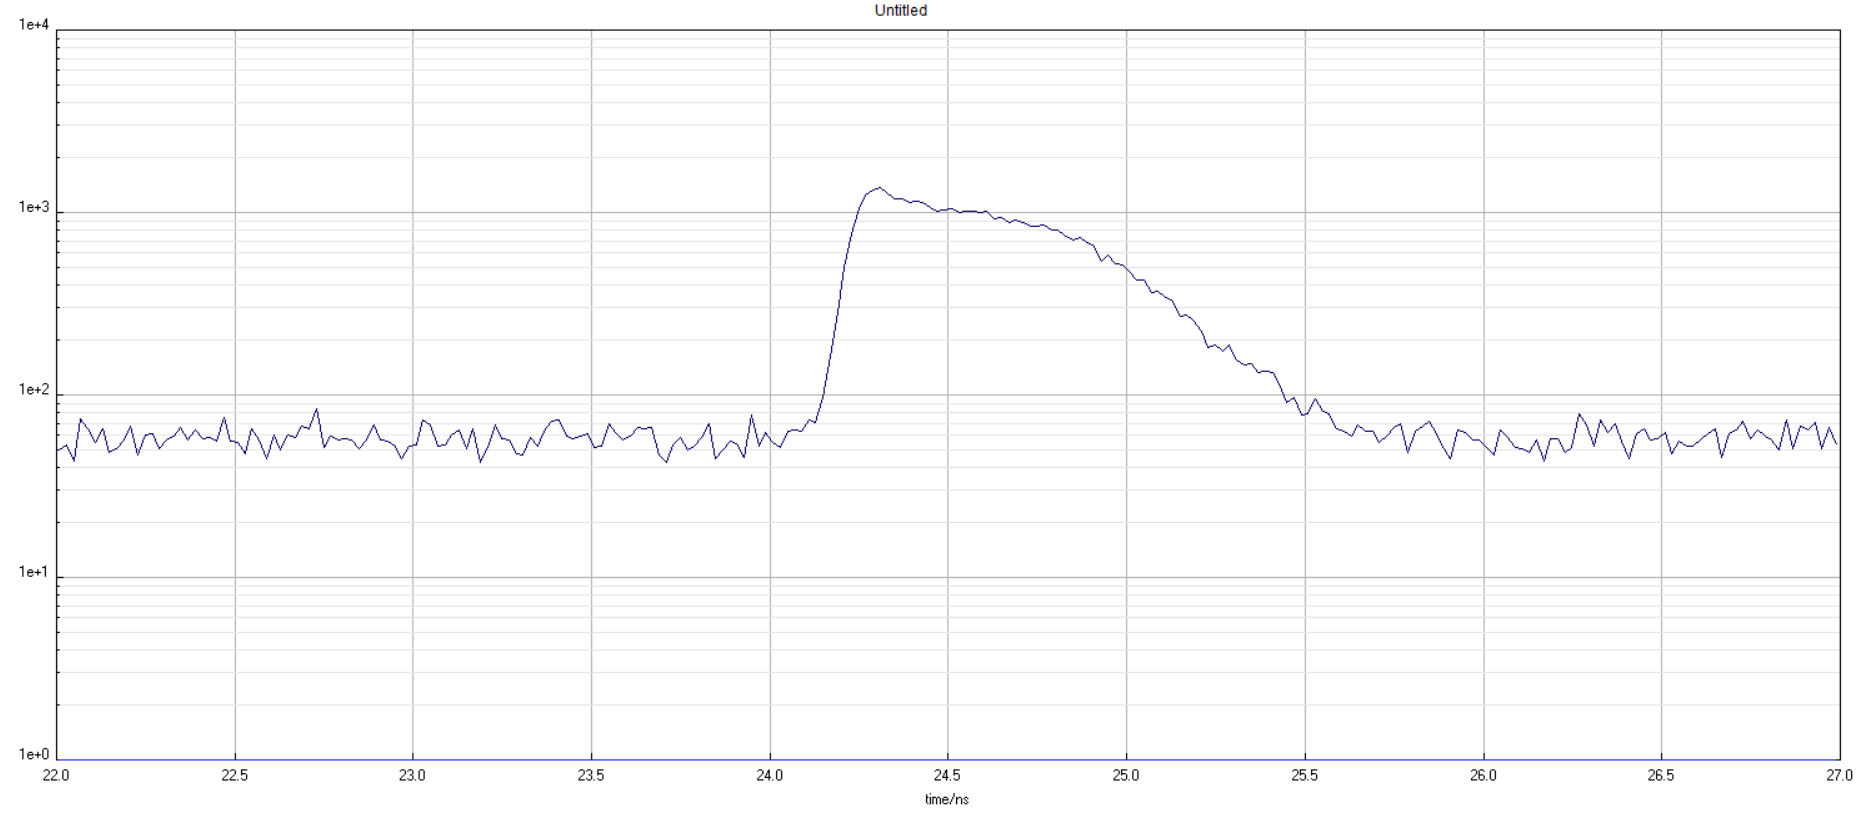
\includegraphics[width=1.0\textwidth]{figures/horiba laser.PNG}
\caption{\label{fig:pulse_1}Pulse measurement with clear temporal dispersion}
\end{figure}

\subsection{Switch to off-table laser}

Due to the dispersion apparent with the Horiba laser, it was decided to switch to the Spectraphysics laser source which had a reliable sync pulse signal. However, this laser at the time was mounted on a separate table, and was unable to be moved due to it's usage in a separate experiment. In order to use the laser, a setup was devised using a multi-mode fiber coupled to the Spectraphysics laser with a simple mount that allowed the laser to shine directly onto the fiber input and couple the beam into it. This fiber was then routed to the original laser table and mounted to have its output shine directly onto a similar sequence of mirrors and and ND filter as before. Fig.\ref{fig:nkt_fiber_coupling} shows the coupling of the Spectraphysics laser into the fiber, which then is routed up through the roof of the lab and then down onto the original laser table as shown in Fig.\ref{fig:fiber_output}

\begin{figure}[!htb]
     \centering
     \begin{subfigure}[t]{0.25\textwidth}
         \centering
         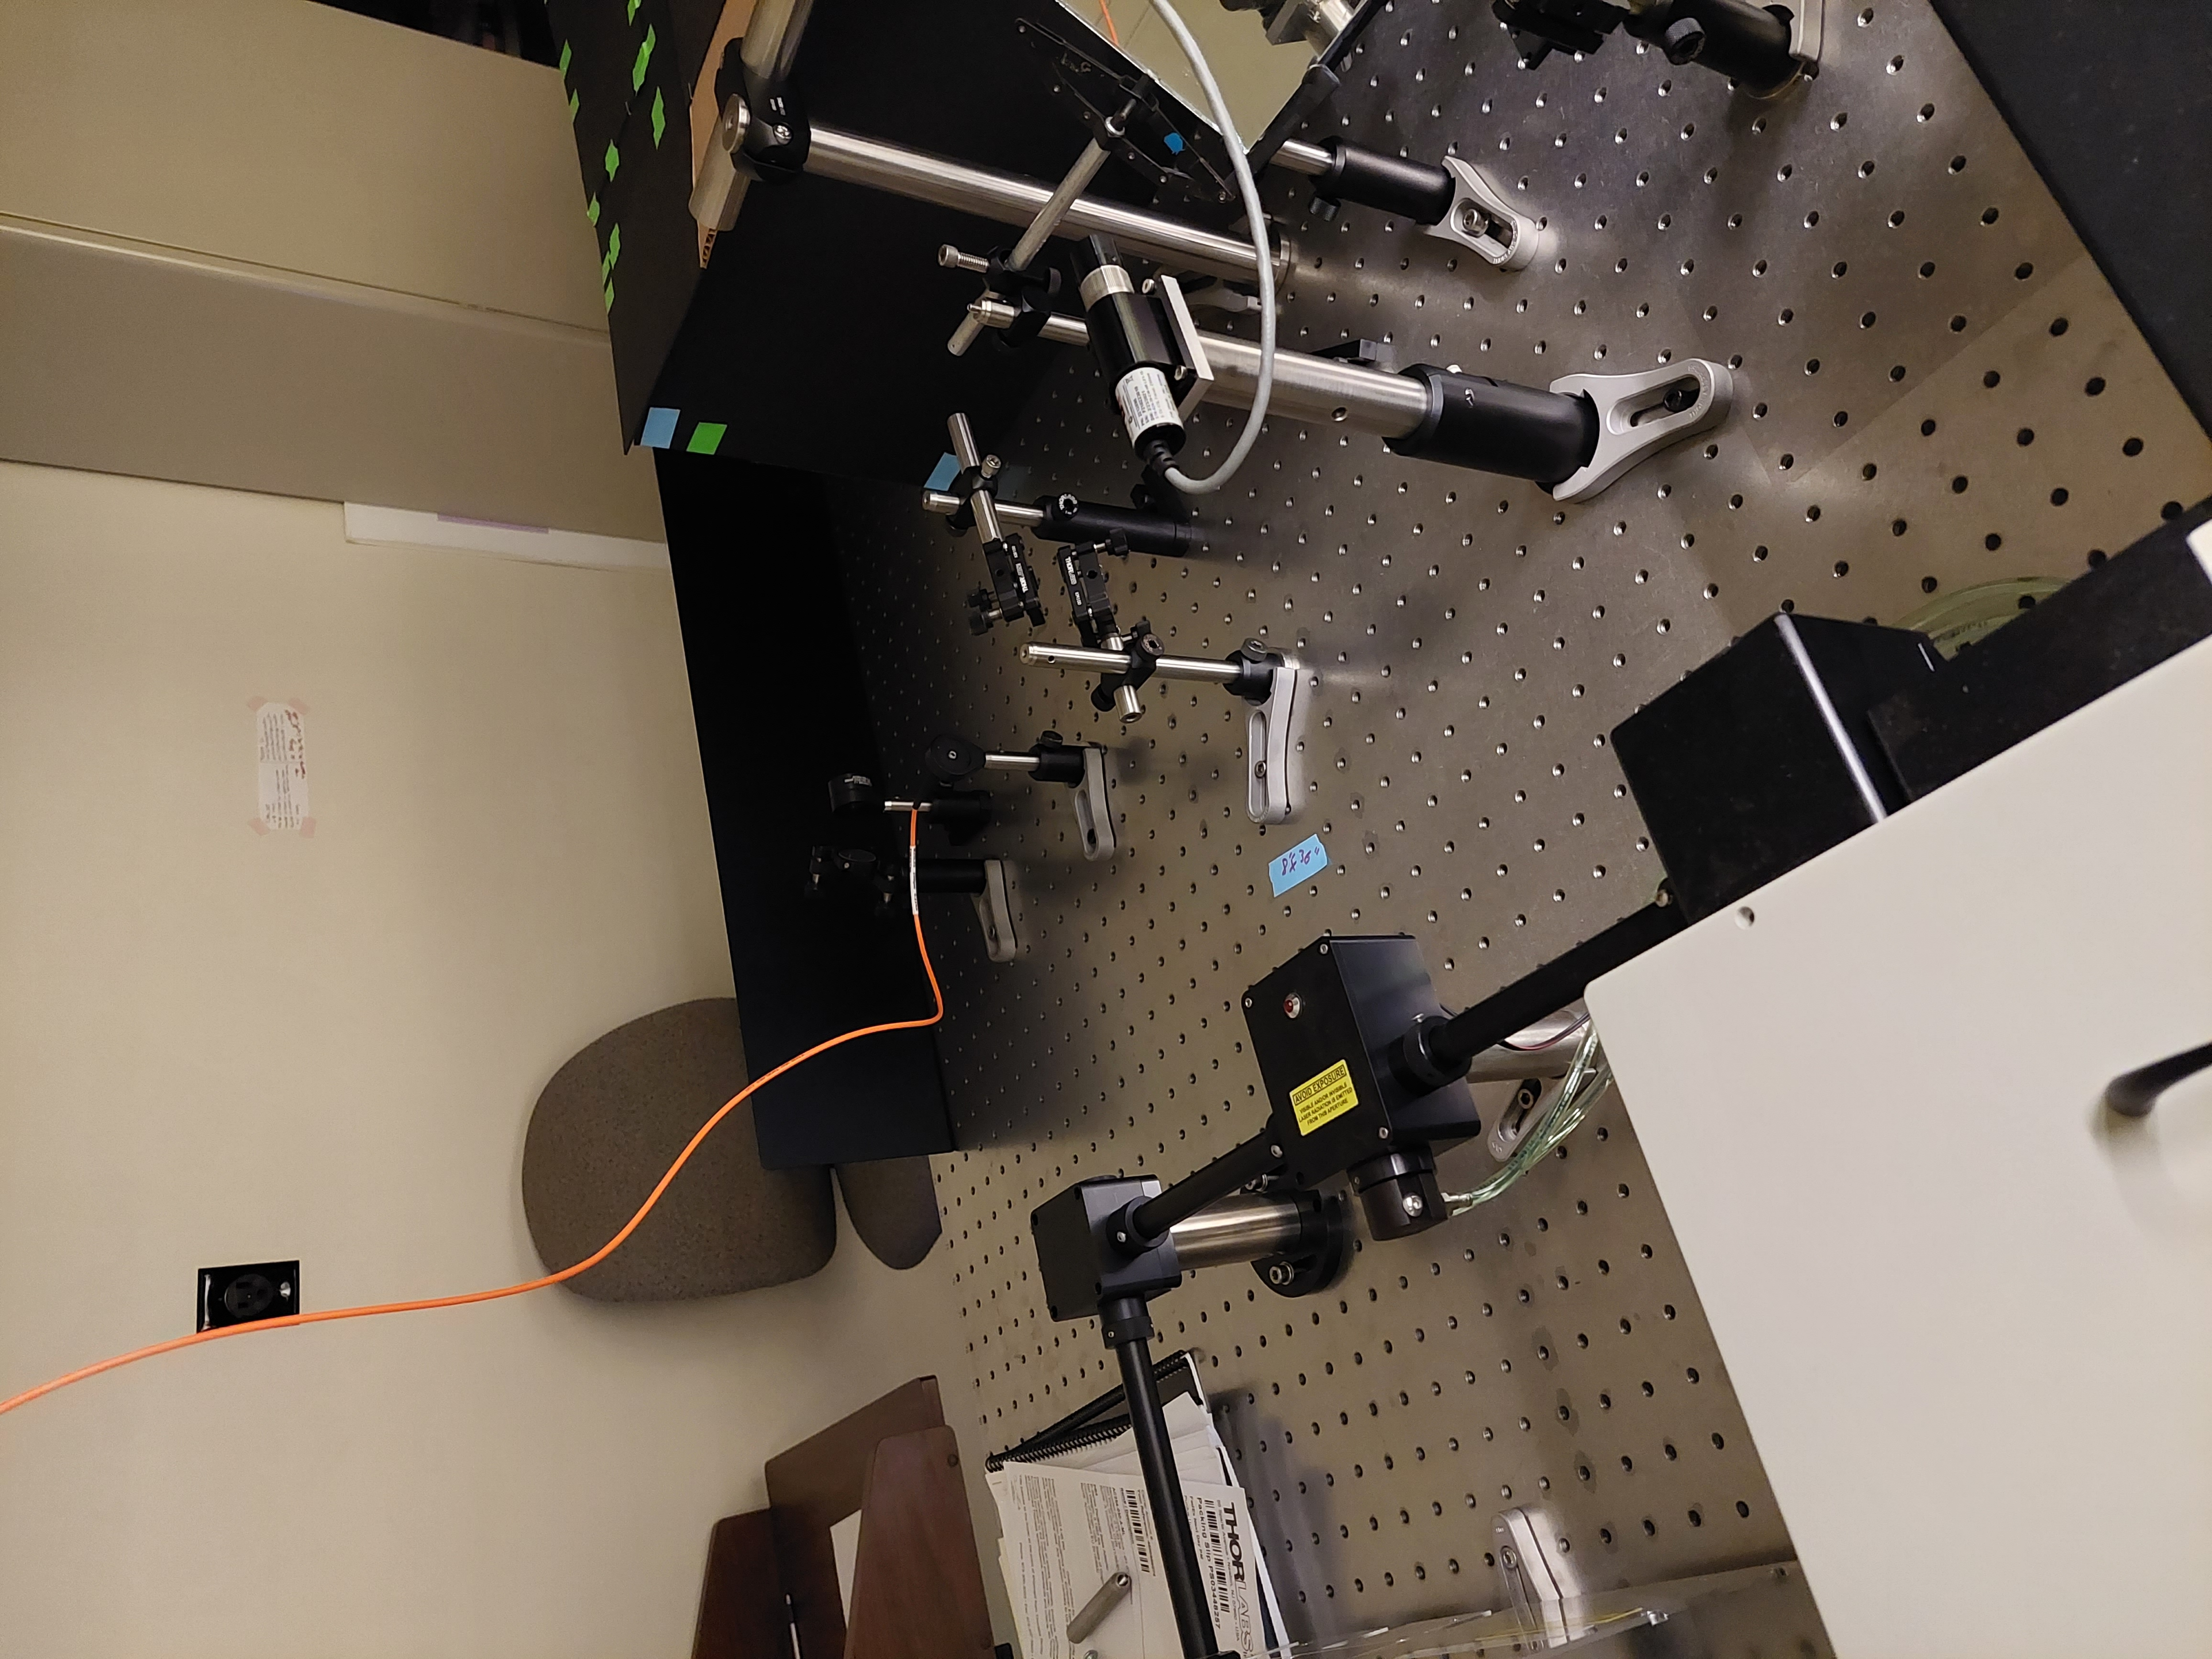
\includegraphics[angle=270,origin=c,width=\textwidth]{figures/20220228_174444.jpg}
         \caption{Fiber coupling setup on separate table}
         \label{fig:nkt_fiber_coupling}
     \end{subfigure}
     \hfill
     \begin{subfigure}[t]{0.25\textwidth}
         \centering
         \includegraphics[angle=270,origin=c,width=\textwidth]{figures/20220228_174340.jpg}
         \caption{Fiber output to photon counting setup}
         \label{fig:fiber_output}
     \end{subfigure}
     \hfill
     \begin{subfigure}[t]{0.4\textwidth}
         \centering
         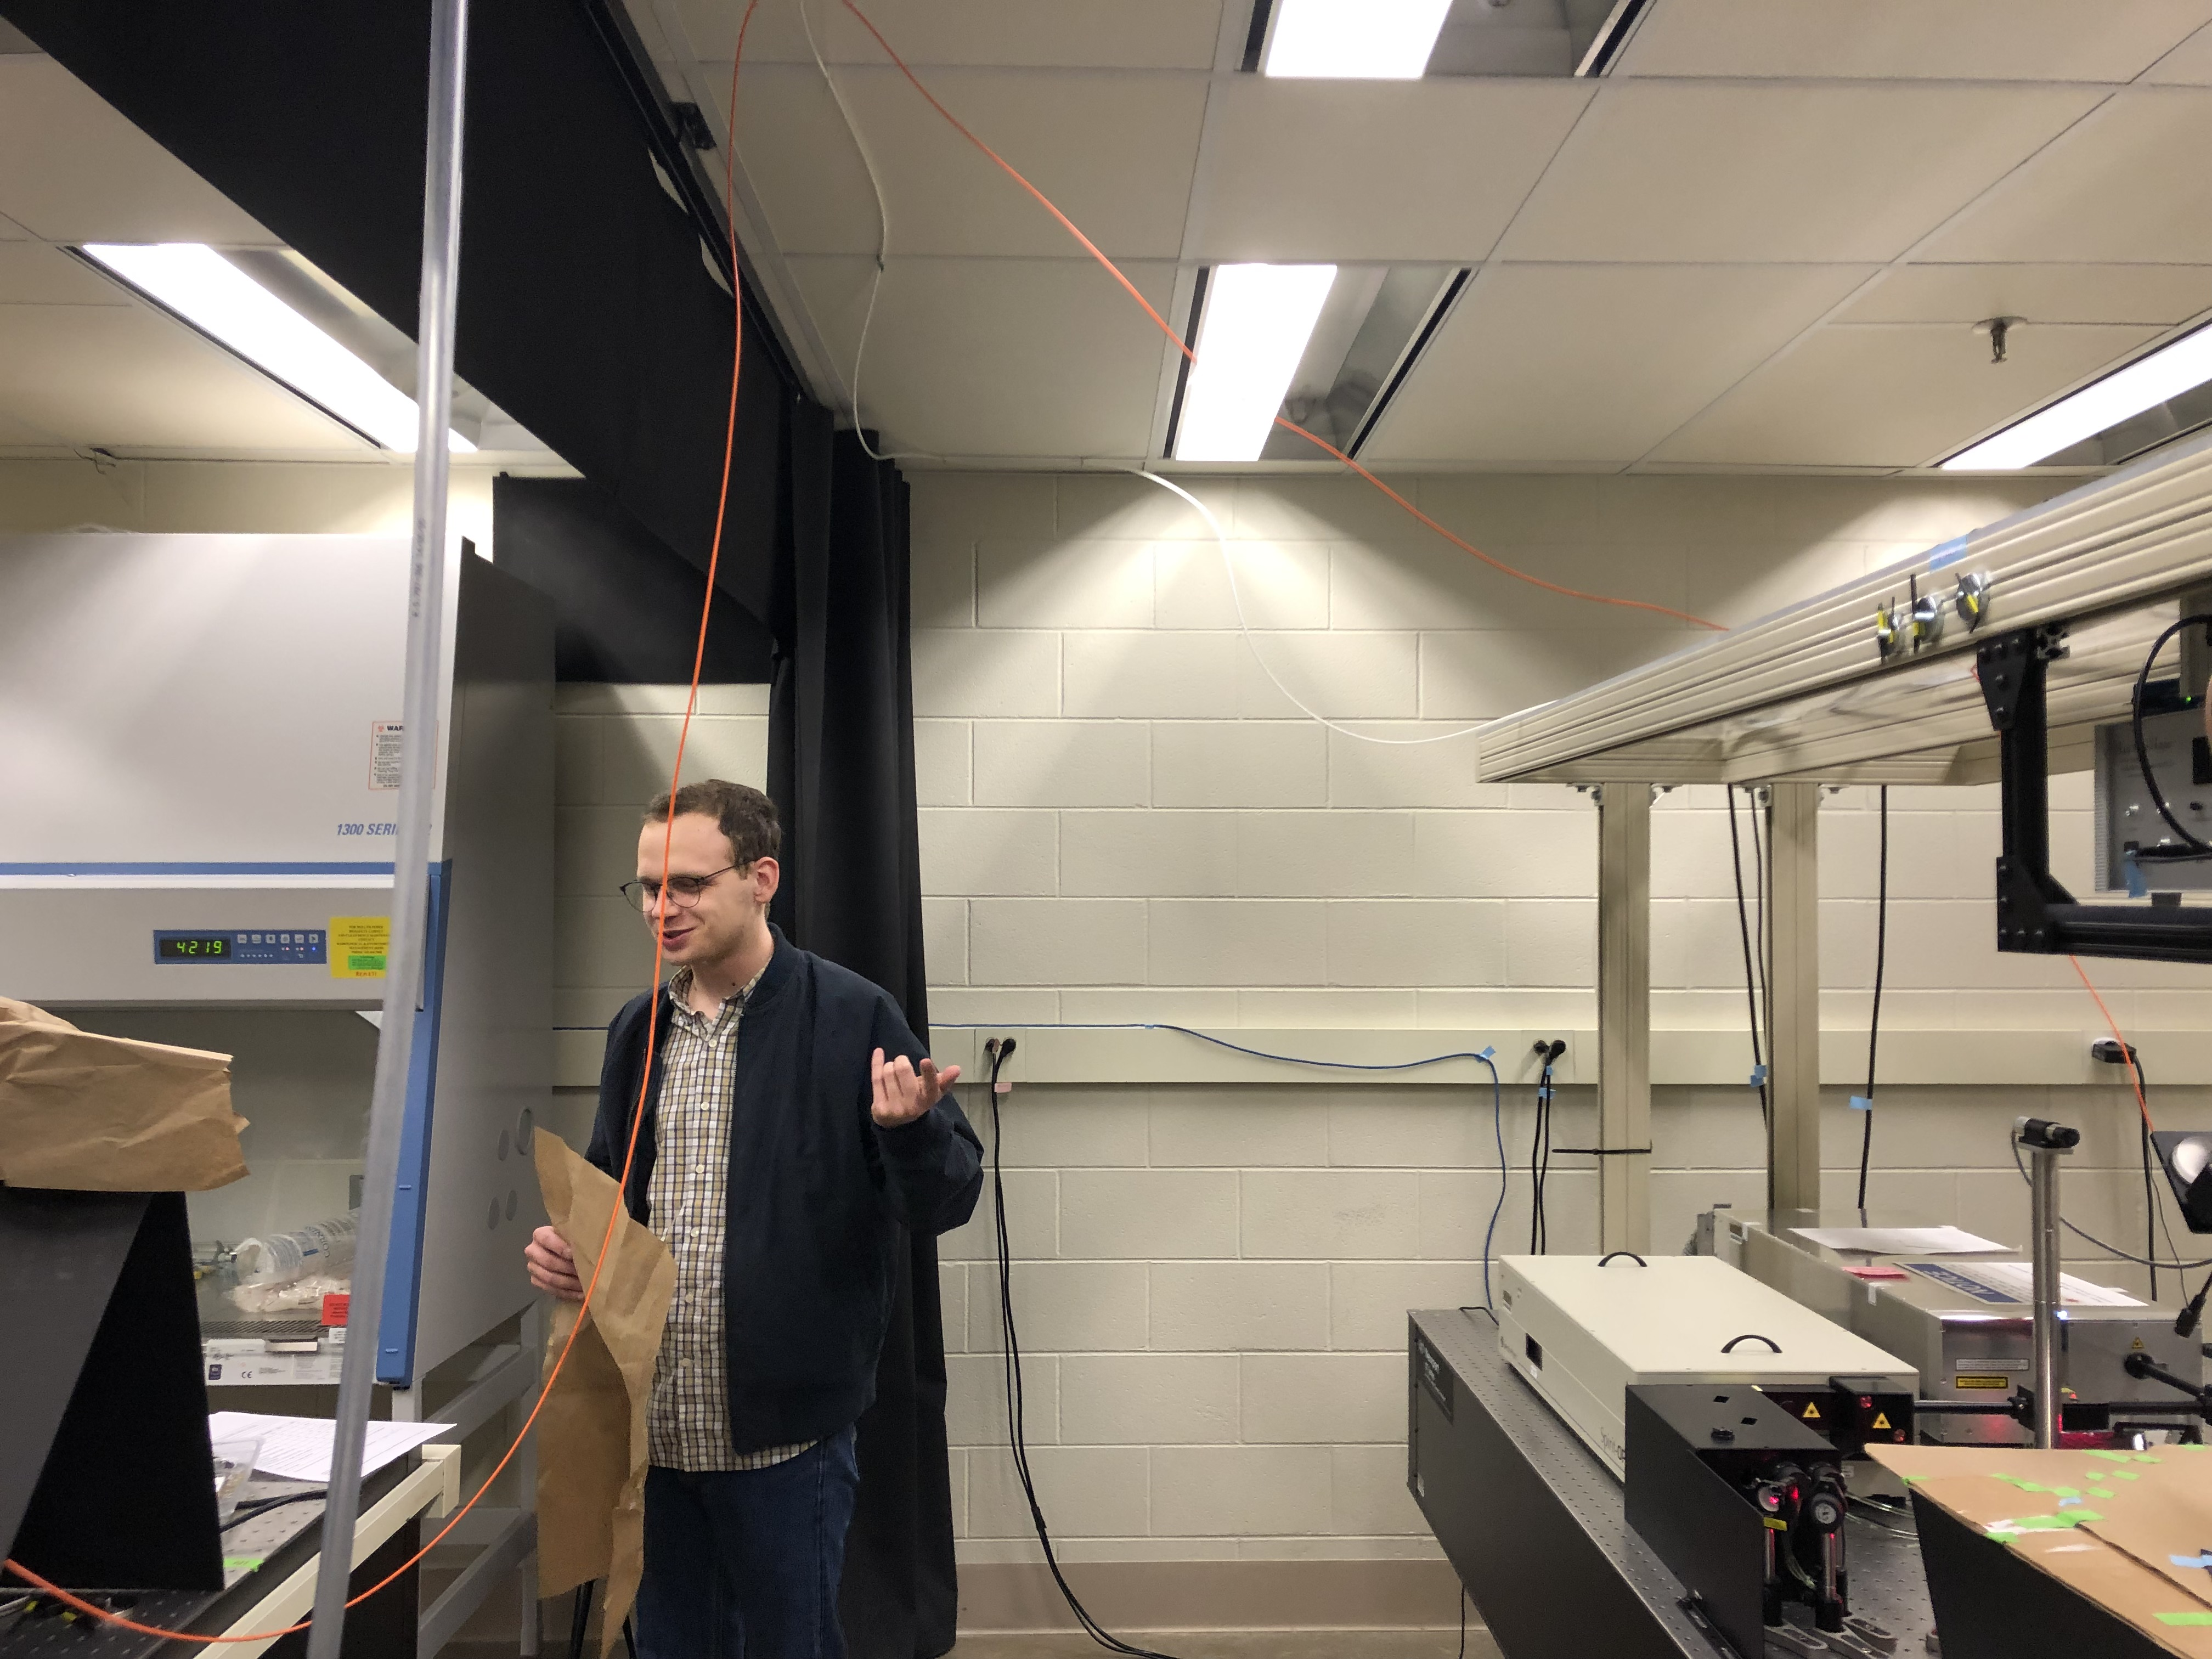
\includegraphics[width=\textwidth]{figures/IMG_6137.jpg}
         \caption{Fiber run through ceiling}
         \label{fig:fiber_ceiling}
         \begin{minipage}{2cm}
         \vfill
         \end{minipage}
     \end{subfigure}
        \caption{Multi-mode fiber setup}
        \label{fig:fiber}
\end{figure}

\subsection{Fiber setup results and issues}

After the hardware setup was complete and the fiber coupling properly, the photon counting hardware was used to analyze the pulse. The resulting graph was not nearly as clean as expected however, and displayed multiple anomalies. First, though the pulse width of the Spectraphysics laser should have been close to 0.4ps, the pulse width seen upon inspection of the photon counting histogram was much larger, and was not symmetric as well as quite noisy.

The first anomaly is that there are 3 separate superimposed pulse shapes in the output as seen in Fig.\ref{fig:fiber_graph_no_hand}. The first is a quick pulse that has almost entirely dropped off before the arrival of the next, widest pulse, followed by a sharp, high amplitude pulse located within the tail of the wide pulse. 

The short beginning pulse was theorized to be cause by laser light coming from the laser table where the Spectraphysics laser was located bouncing off optical elements and the white back wall and then into the SPAD aperture. Because the fiber was coupled on the table in an open environment with many different optical paths (the Spectraphysics source was split and used for multiple experiments simultaneously), there was a significant amount of scattered laser light illuminating the back wall, apparent very clearly by eye. The short initial pulse was suspected as being the pulse caused by the reflected laser light because it arrives first, meaning the light took less time to arrive at the aperture. Due to the nature of the fiber, and its significant length, the pulse would take longer to travel through the fiber and into the aperture than to only bounce off the wall and across the tables into the aperture.

To test whether this scattered light from the table was the cause of the early initial pulse, the aperture was shielded from any laser light coming from any source other than the fiber. Initially, a person stood between the two tables to block the non-fiber light, and the resulting histogram was Fig.\ref{fig:fiber_graph_hand}. It clearly shows an almost complete removal of the initial pulse. The cross-table bounce then serves as a satisfactory explanation for the initial pulse, however the 2 other pulses must now be accounted for.

The suspected cause of the 2 other pulses is modal dispersion, as the fiber used was a multi-mode fiber. An additional factor leading this to be suspected is that upon close visual inspection of the laser light output from the fiber, multiple different interference patterns were visible, indicative that the laser pulse was exciting multiple modes within the fiber simultaneously. The result of such multi-mode propagation is that, due to differences in propagation velocity of different modes, the arrival time of the pulse carried by each mode will be different, and the output will be the superposition of each mode's transmission.

%
%Put the multi-mode fiber analysis
%

A more elaborate shielding setup was devised using black cardstock to cover the SPAD, however the multi-mode dispersion was not able to be reduced and so the setup was unsatisfactory.

\begin{figure}[!htb]
     \centering
     \begin{subfigure}[b]{1.0\textwidth}
         \centering
         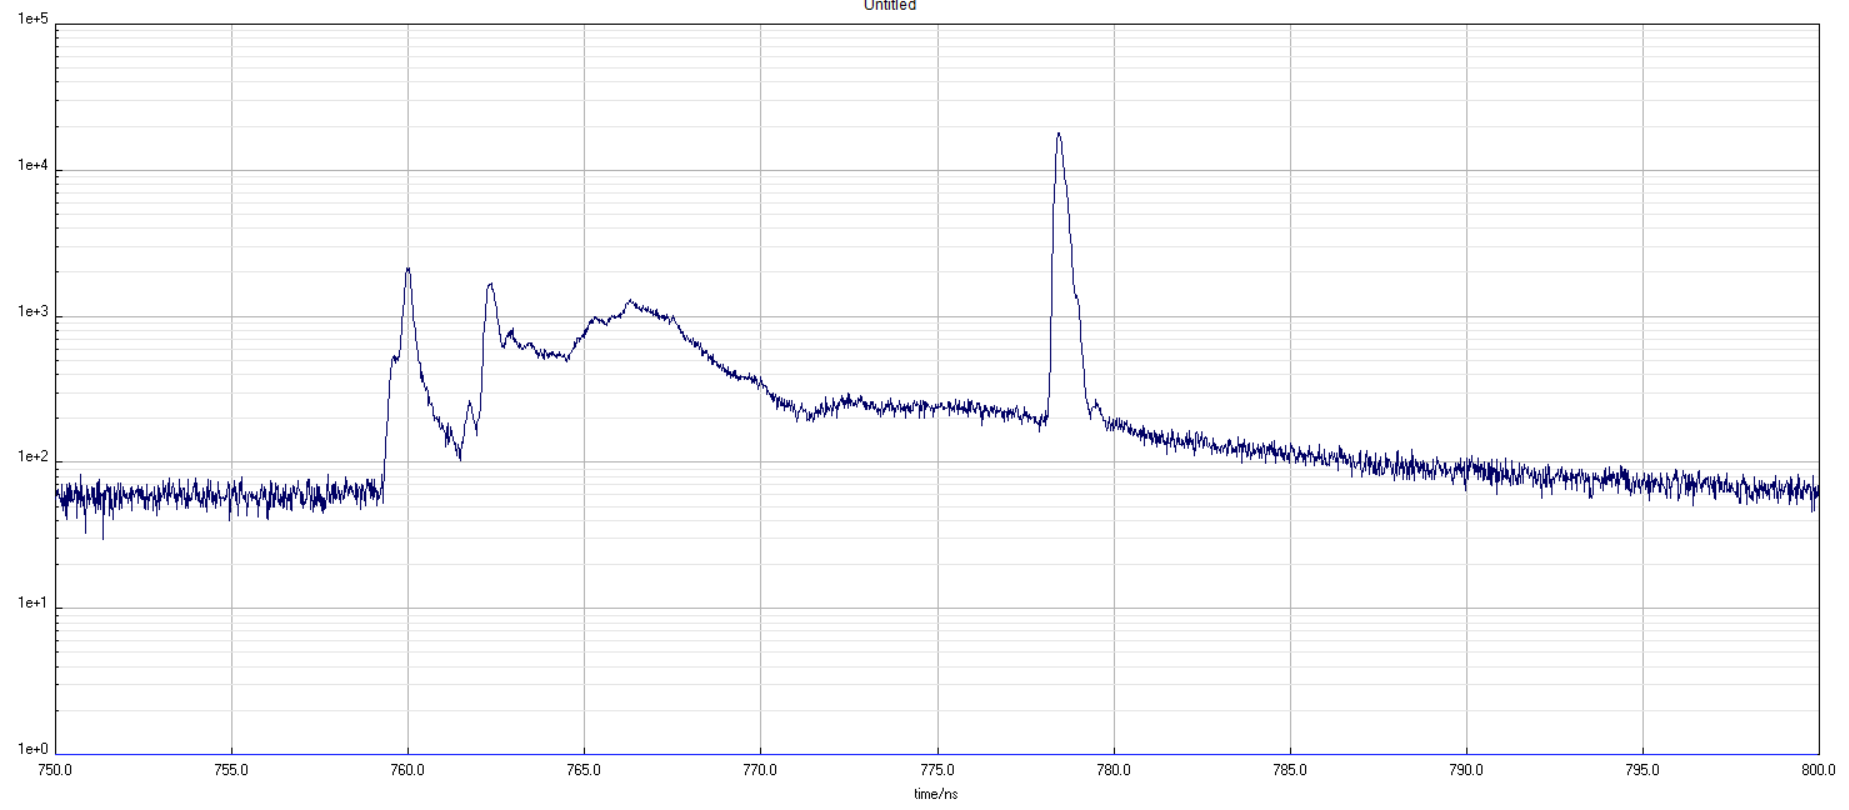
\includegraphics[width=\textwidth]{figures/550_no_hand.PNG}
         \caption{Histogram results with no shielding}
         \label{fig:fiber_graph_no_hand}
     \end{subfigure}
     \hfill
     \begin{subfigure}[b]{1.0\textwidth}
         \centering
         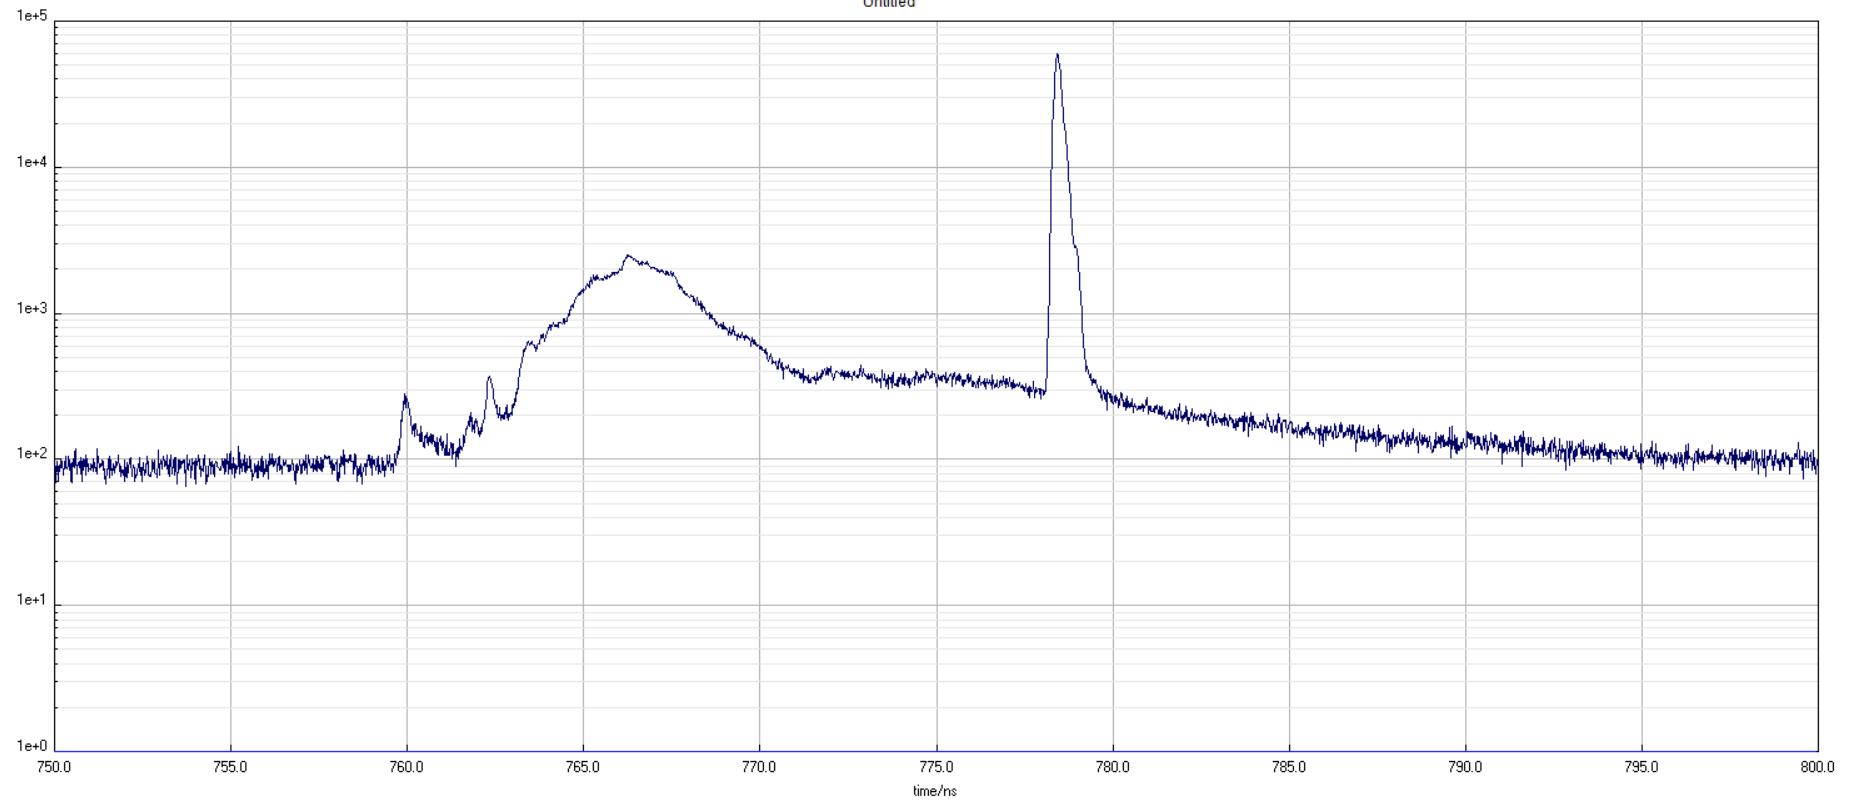
\includegraphics[width=\textwidth]{figures/550-actually covered.PNG}
         \caption{Histogram with shielding}
         \label{fig:fiber_graph_hand}
     \end{subfigure}
        \caption{Multi-mode fiber  back-reflection and dispersion}
        \label{fig:fiber_graphs}
\end{figure}

\subsection{Setup with NKT laser on same table}

After the issues with the previous setup due to coupling with the fiber causing spreading, and an NKT laser being freed up from its previous usage in another setup, the NKT laser was moved to the same table as where the photon counting equipment and SPAD reside. This allowed the laser pulse to be routed directly from the output aperture through just a few optical elements before arriving at the SPAD detector.

Beneath the laser table was placed the NKT super-continuum laser source shown in Fig.\ref{fig:super_continuum}, with the laser signal routed up to the table to a variable band-pass filter in Fig.\ref{fig:band_pass}, allowing the entire setup to act as a variable wavelength narrow-band laser source.

\begin{figure}
     \centering
     \begin{subfigure}[b]{0.48\textwidth}
         \centering
         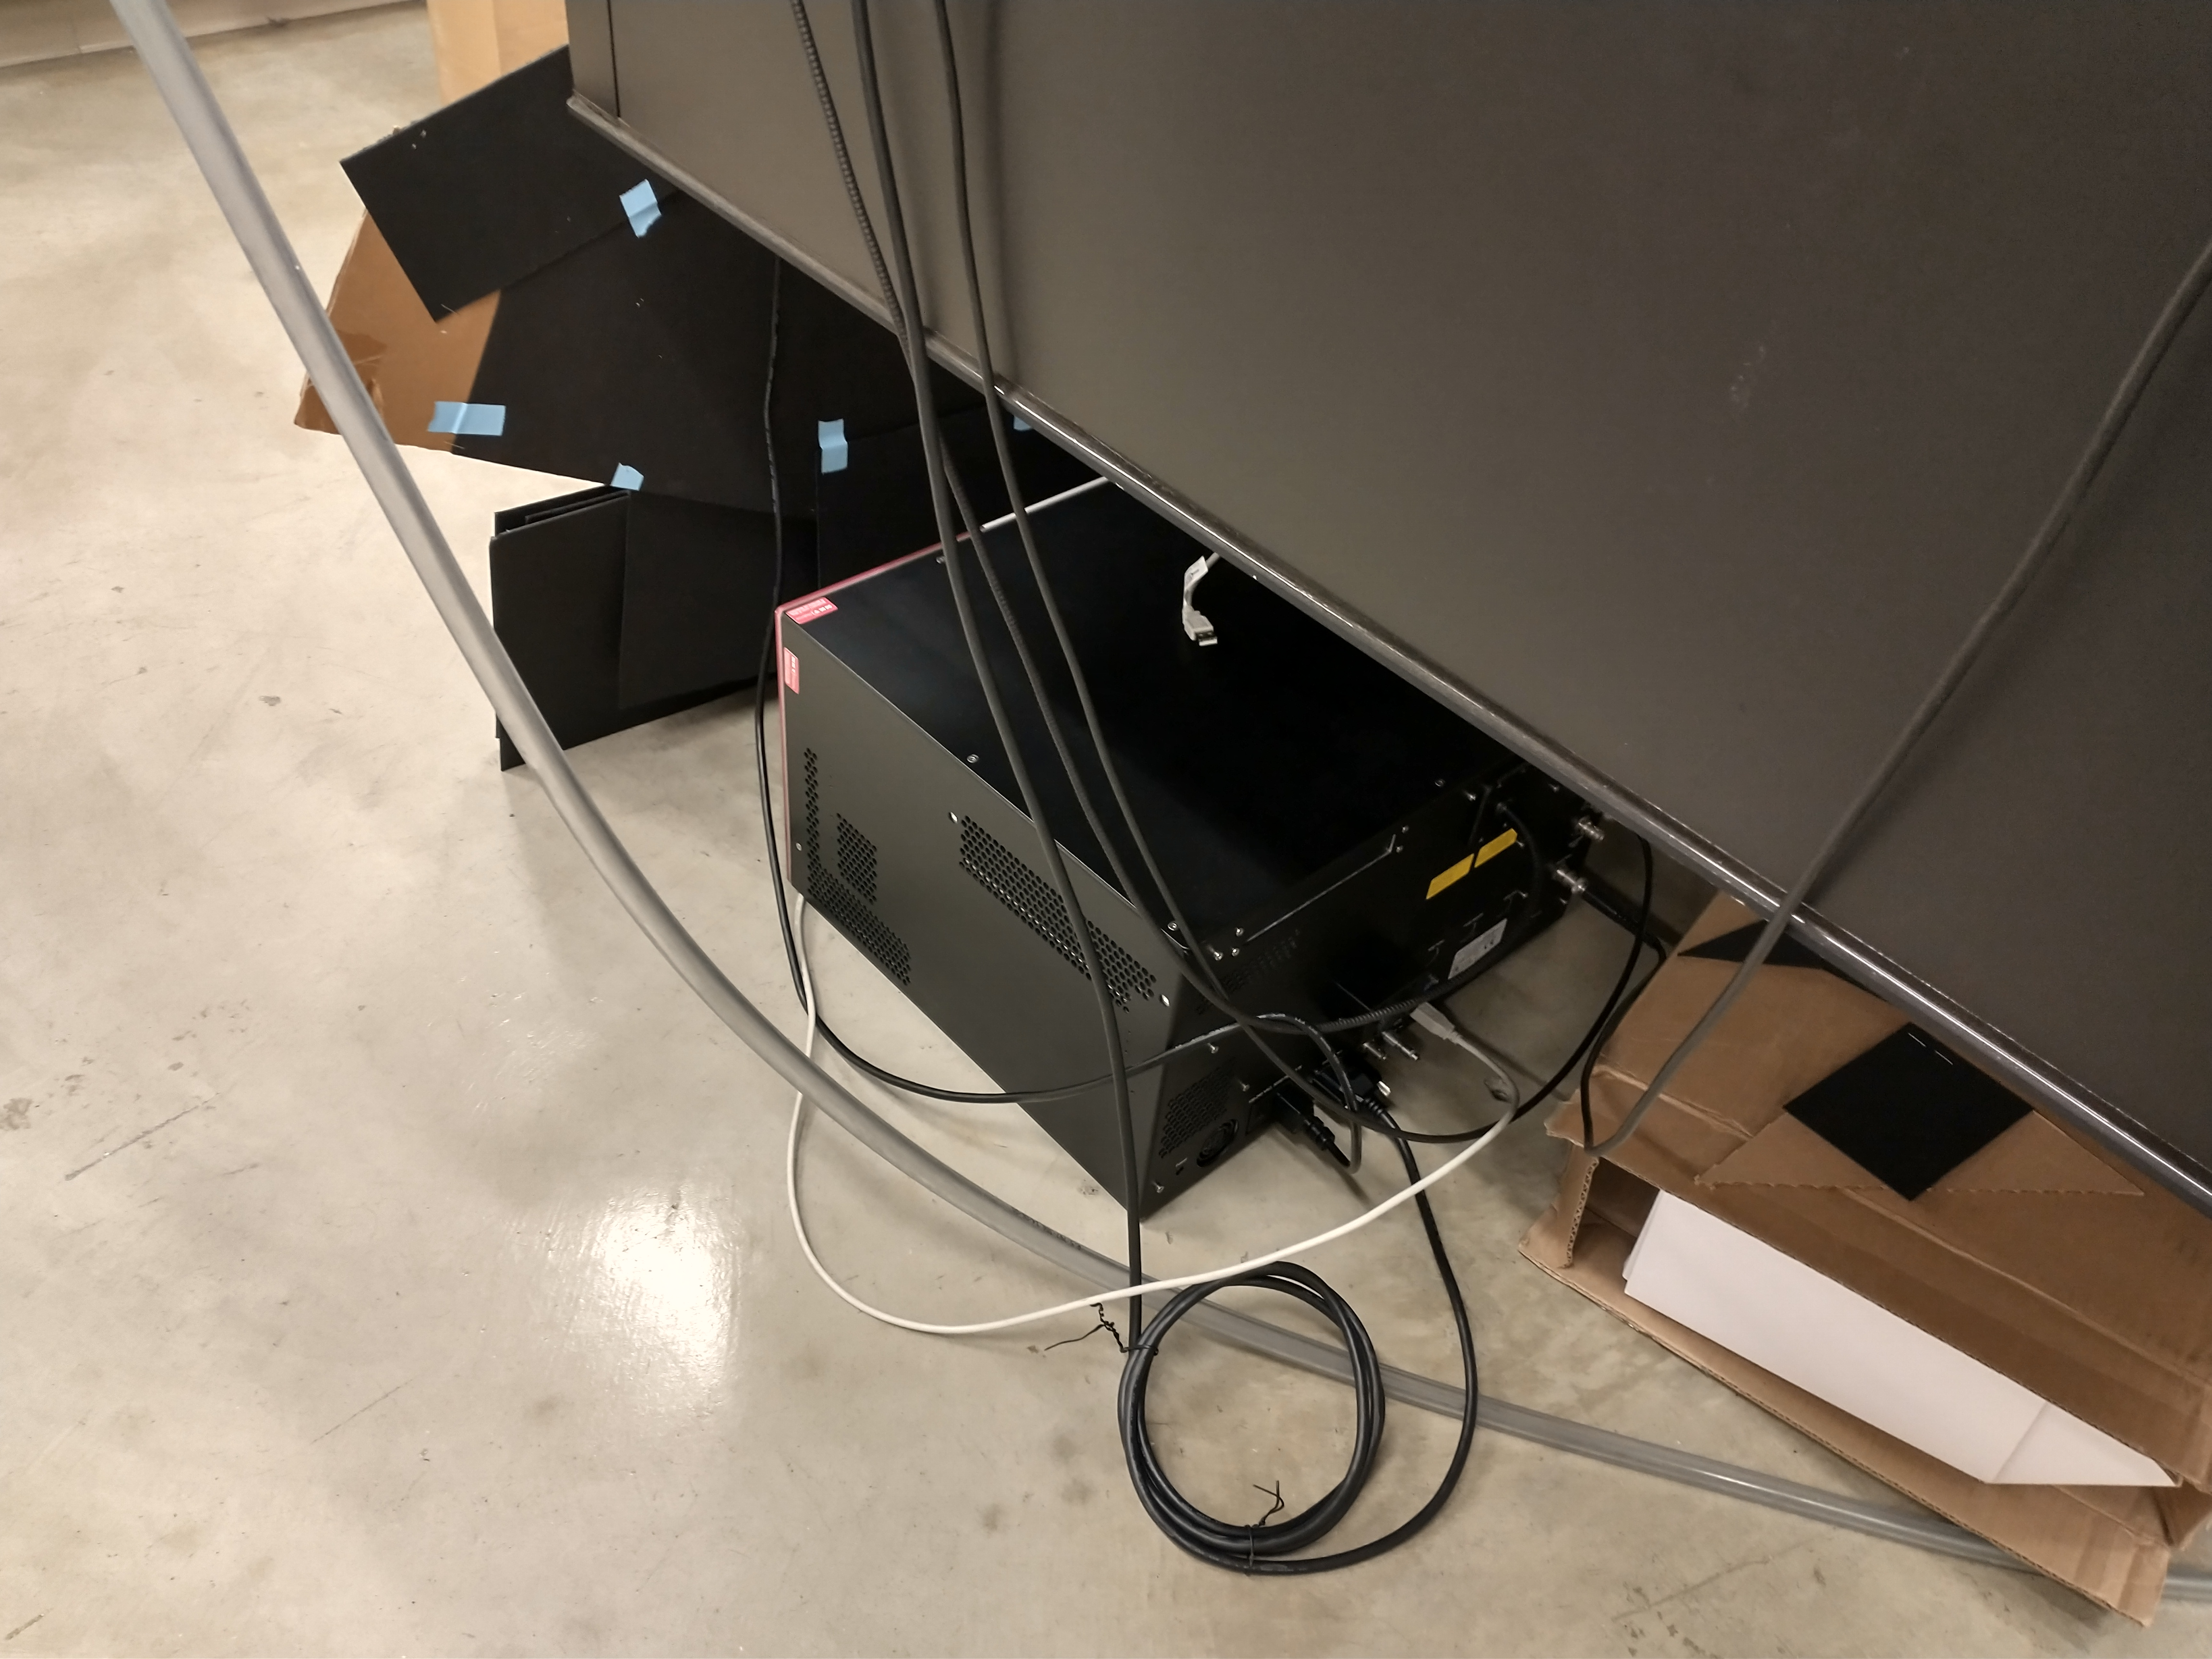
\includegraphics[width=\textwidth]{figures/IMG_20220422_134723634_HDR.jpg}
         \caption{NKT super-continuum laser source}
         \label{fig:super_continuum}
     \end{subfigure}
     \hfill
     \begin{subfigure}[b]{0.48\textwidth}
         \centering
         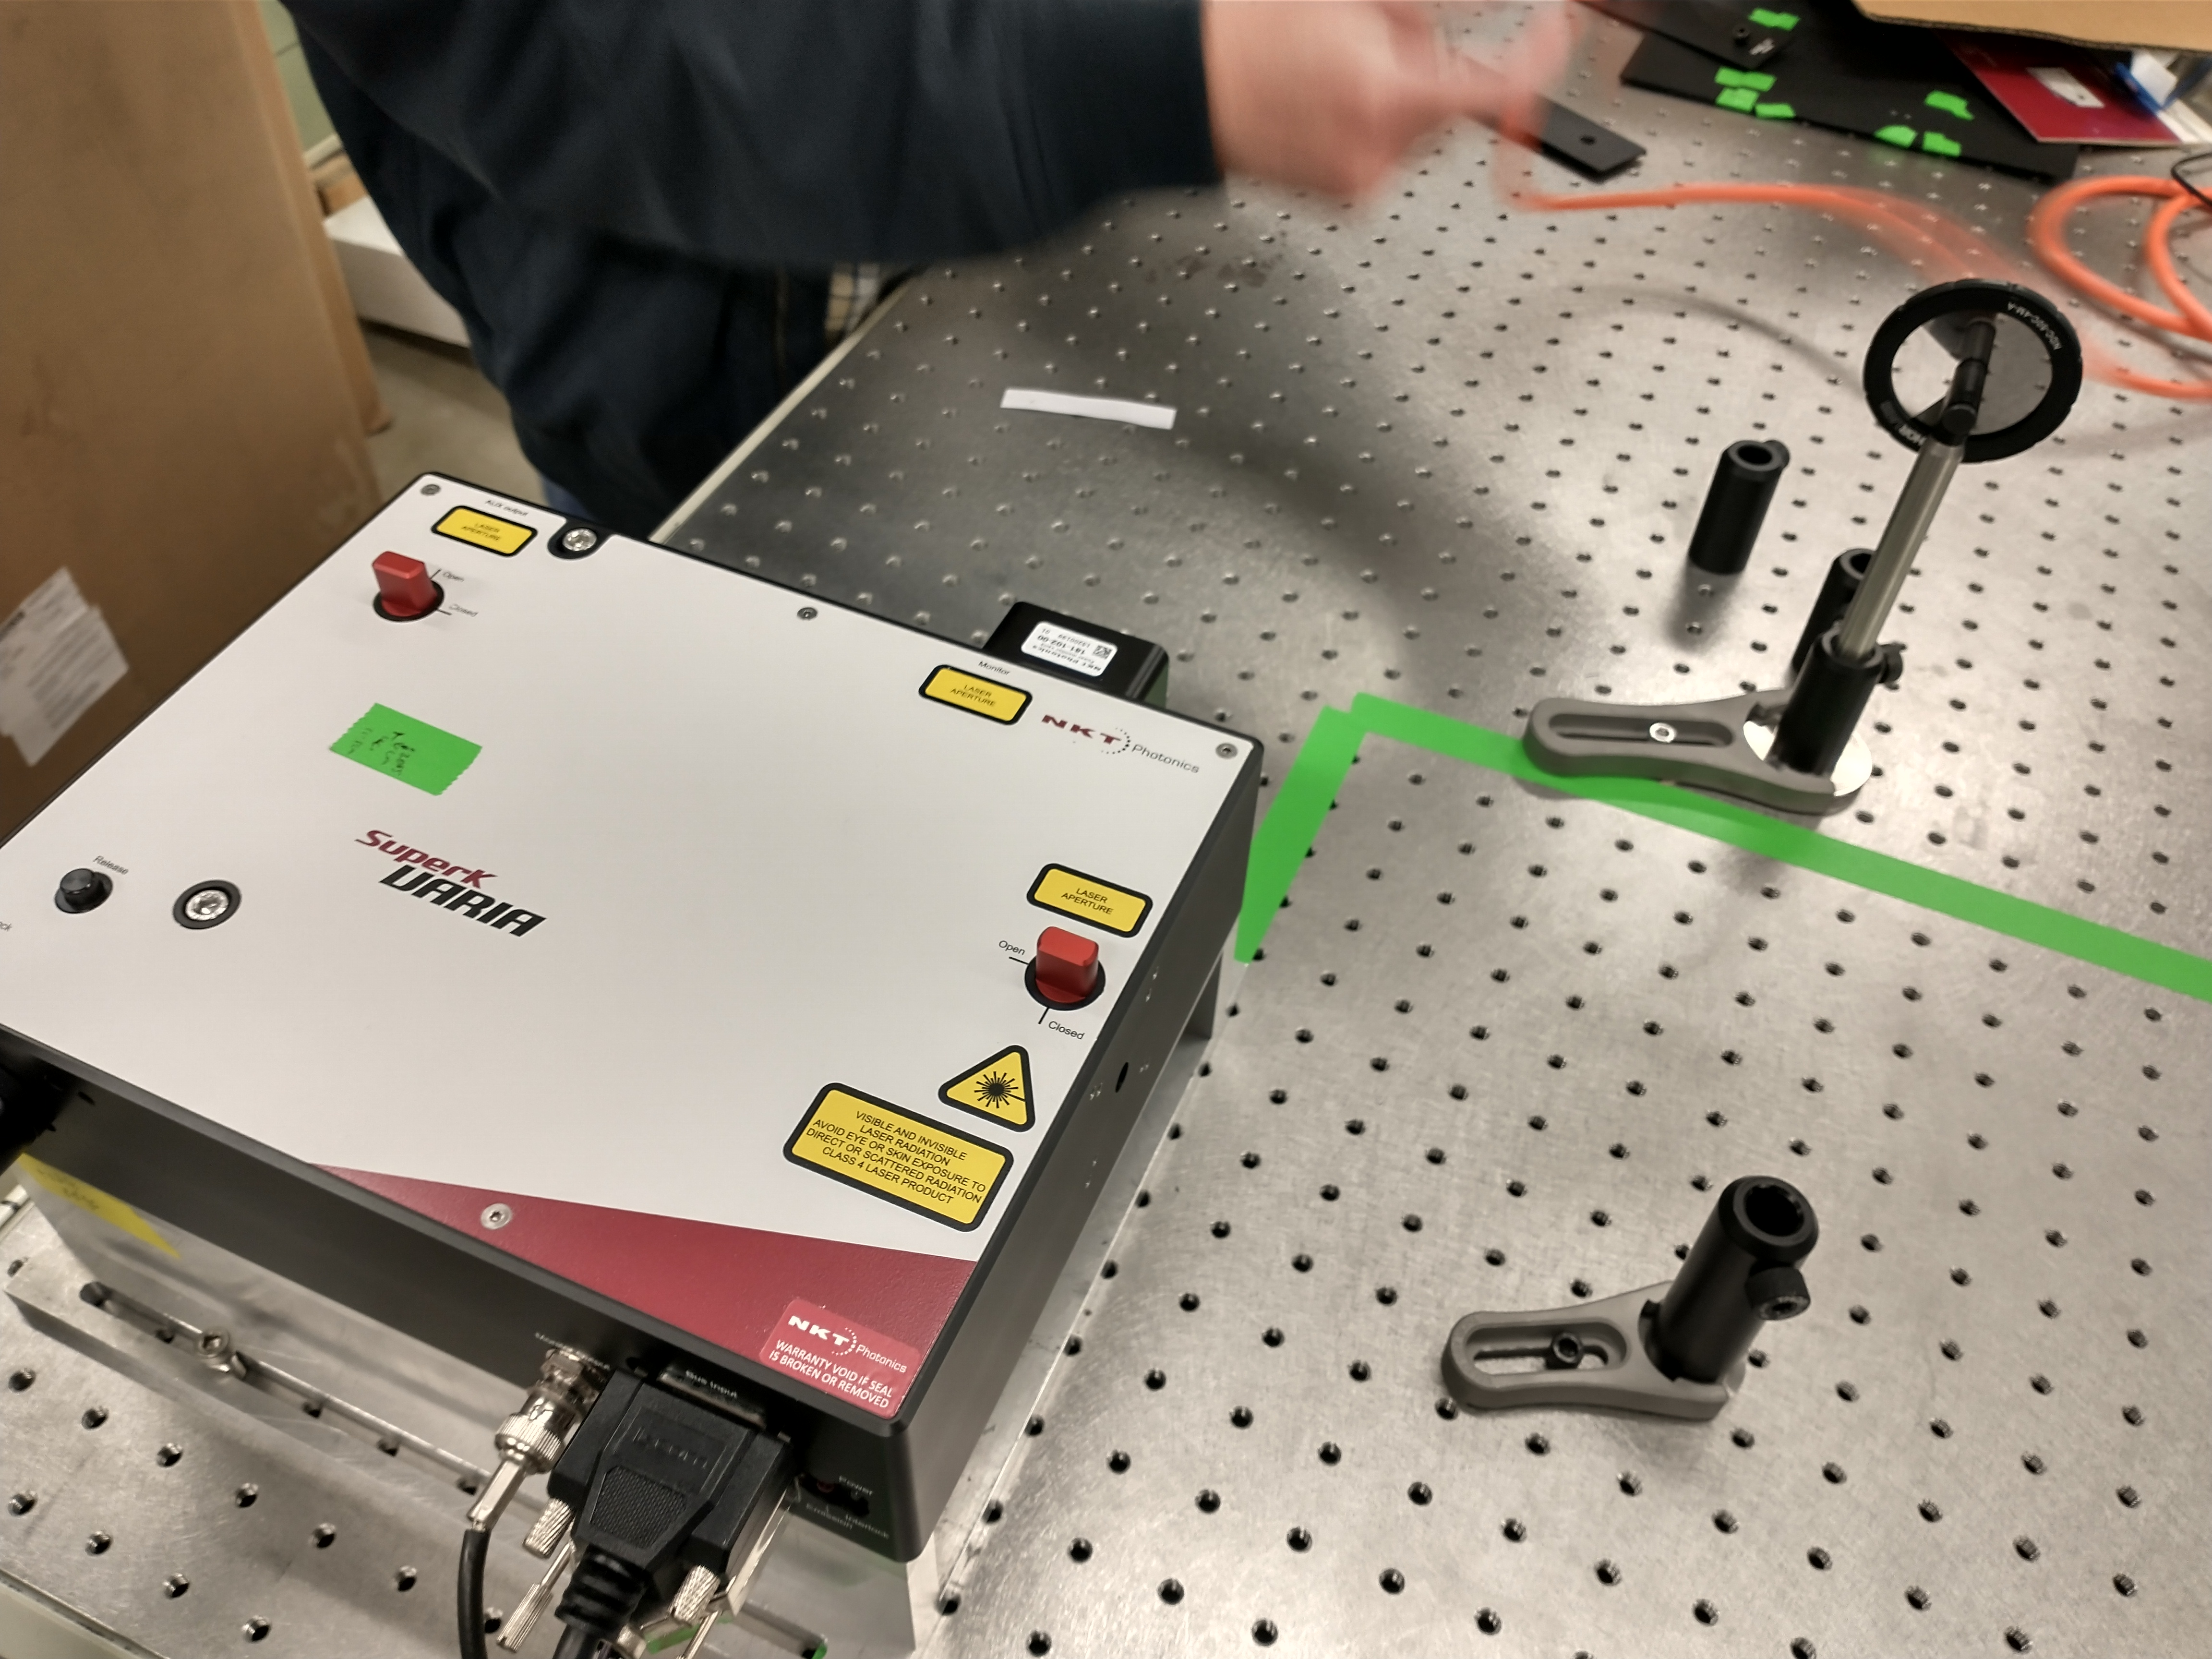
\includegraphics[width=\textwidth]{figures/IMG_20220422_134731107_HDR.jpg}
         \caption{NKT SuperK Varia band-pass filter}
         \label{fig:band_pass}
     \end{subfigure}
        \caption{NKT laser}
        \label{fig:NKT_laser_setup}
\end{figure}

The output of the laser from the band-pass filter was then directed into a beam collimator, 45deg mirror, and an ND filter before being directed into the SPAD aperture. It was not possible to find posts such that the laser output and the SPAD aperture would be on the same horizontal plane, so the collimator we adjusted to direct the beam upward so that the vertical differential was removed. With the ND filter properly adjusted such that the probability of arrival of a photon within a pulse was below the recommended threshold, the setup was ready for measurement.

The complete setup is shown in Fig.\ref{fig:nkt_same_table}.
Measurement results were recorded and shown in Fig.\ref{fig:python_graph}.

\subsection{Initial Results}

The measurement resulting from this experimental setup appear much cleaner and more symmetrical than previous setups, with the pulse width appearing much shorter. As opposed to previous results, the measured waveform is mostly gaussian and nearly symmetrical, which is desired as that is the shape of the pulsed laser directed at the SPAD aperture. Although much narrower than previous experiments, it does not appear to be in the range of the 5ps pulse width of the NKT laser used in this experiment.

\begin{figure}
\centering
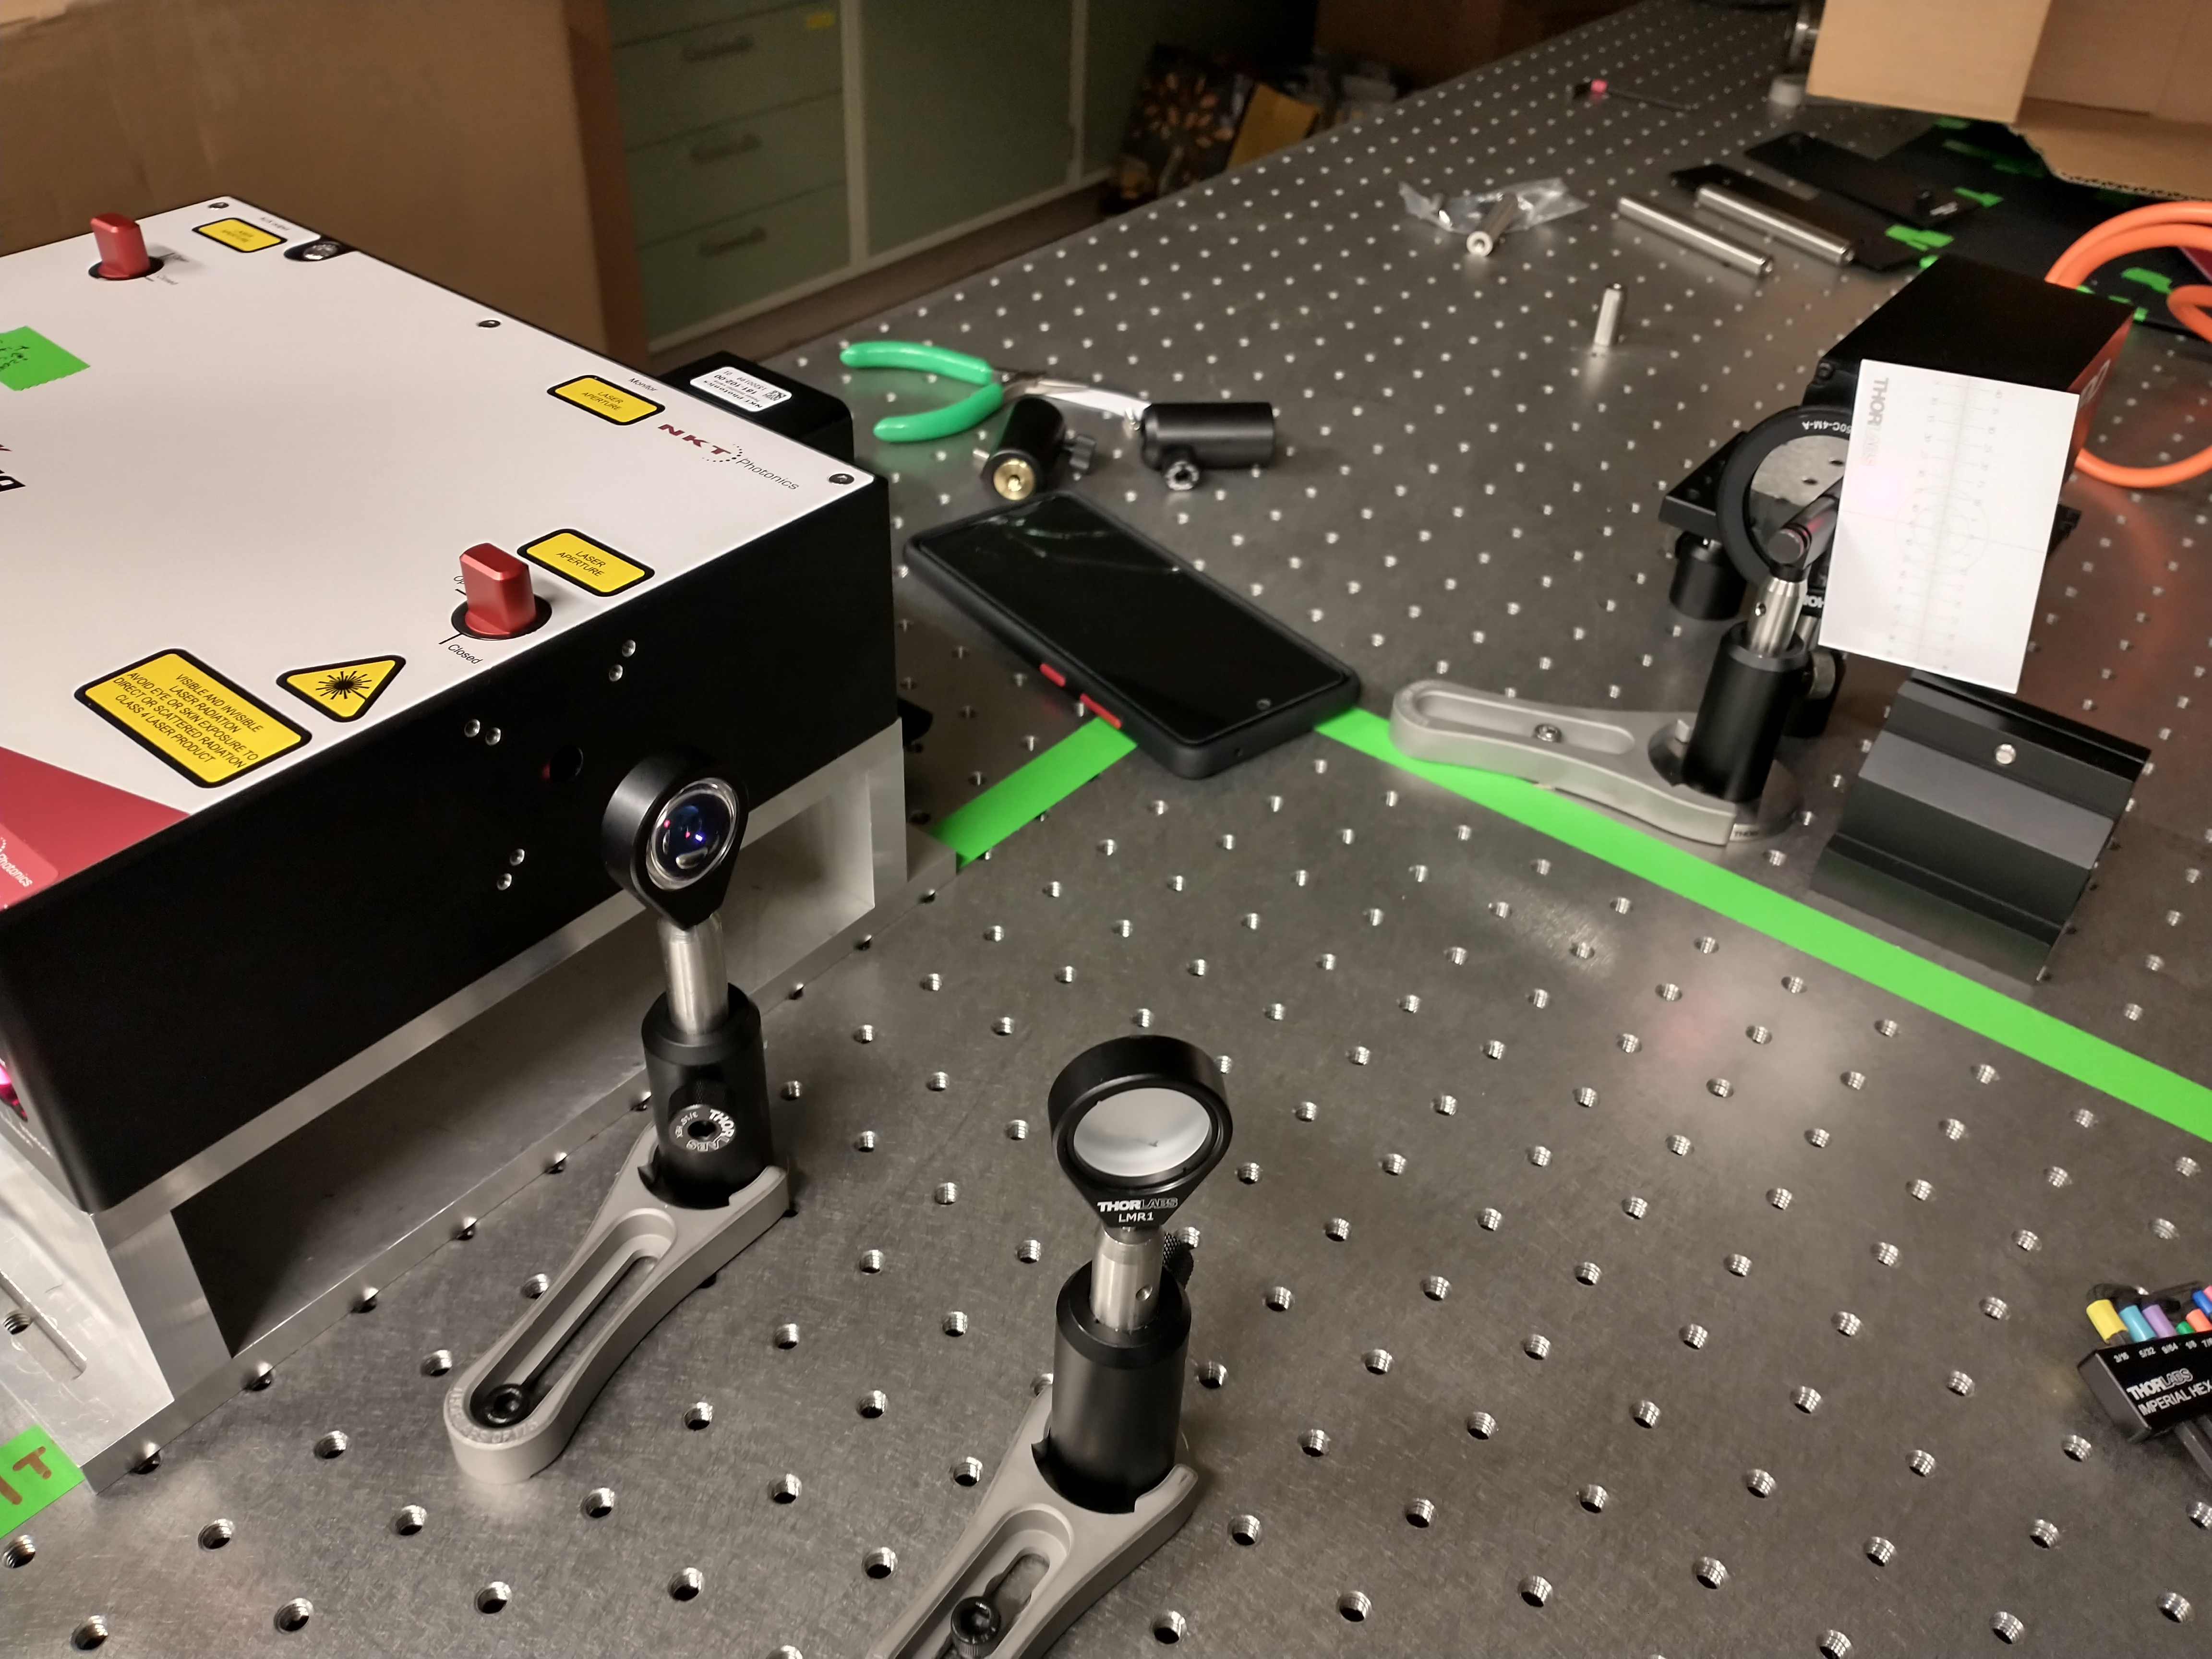
\includegraphics[width=0.6\textwidth]{figures/IMG_20220422_142651049_HDR.jpg}
\caption{\label{fig:nkt_same_table}NKT laser full setup}
\end{figure}

\begin{figure}
\centering
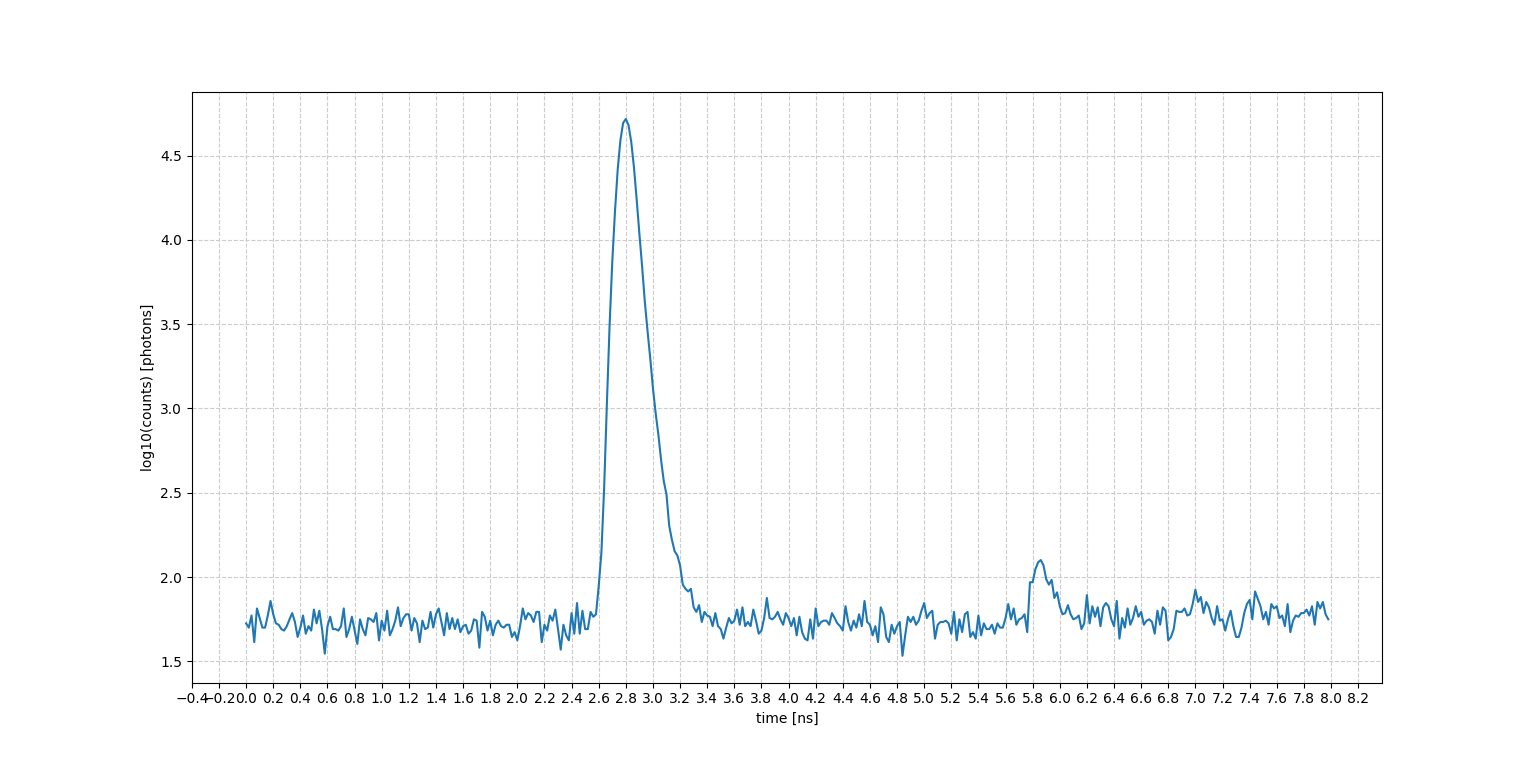
\includegraphics[width=1.0\textwidth]{figures/python_pulse_graph.png}
\caption{\label{fig:python_graph}Pulse histogram from python script}
\end{figure}

\subsection{Full width half max measurement}

In order to better characterize the laser pulse, the histogram data from the SPAD measurement was passed through a custom python script to calculate the FWHM of the pulse.
Using the data exported from the SPAD histogram measurement, the python script finds the maximum pulse amplitude, in histogram counts, and then the timestamps of the bin counts with half of the maximum counts.

The script takes as an input the .dat file generated by the photon counting control software, which contains the raw photon count data and binning units needed to properly reproduce the histogram. The script then generates from the a plot of the histogram as well as a automatically calculated FWHM measurement. Fig.\ref{fig:python_graph} shows the resulting plot of the histogram for this measurement and setup. Below is the console output of the script, displaying intermediate measurements as well as the final FWHM measure

\begin{verbatim}
ns per bin:             0.02 [ns]
min_index:              138
max_index:              143
max_count:              52169
full_width_half_max:    0.1 [ns]
\end{verbatim}

The result of this analysis is a FWHW of 100 ps. The advertised FWHM pulse duration of the laser at \(\lambda\) = 635nm is 5ps, so clearly there must be some dispersive error, or measurement error.

\subsection{Temporal dispersion \& error origin analysis}

Upon review of the laser pulse measurement, there is a clear disparity between the measured pulse width and the advertised pulse width from the laser manual, as the measured pulse width is 100ps, and the advertised width is 5ps. A possible reason for this is temporal dispersion caused by photons bouncing off of the ND filter in front of the SPAD aperture and then off other optical equipment, and then back into the SPAD.

To investigate this, the dimensions of the most likely bounce path were measured and the traversal time the would elapse for it to cover that distance were calculated.
The most likely bounce path appears to be approx. 20 inches, based off a 1 inch hole spacing on the laser table, and the path as shown in Fig.\ref{fig:light_path_measured}.

%
% [!htb]
%

\begin{figure}
     \centering
     \begin{subfigure}[b]{0.49\textwidth}
         \centering
         \includegraphics[width=\textwidth]{figures/IMG_20220422_142643396_HDR.jpg}
         \caption{Possible light bounce path}
         \label{fig:light_path}
     \end{subfigure}
     \hfill
     \begin{subfigure}[b]{0.49\textwidth}
         \centering
         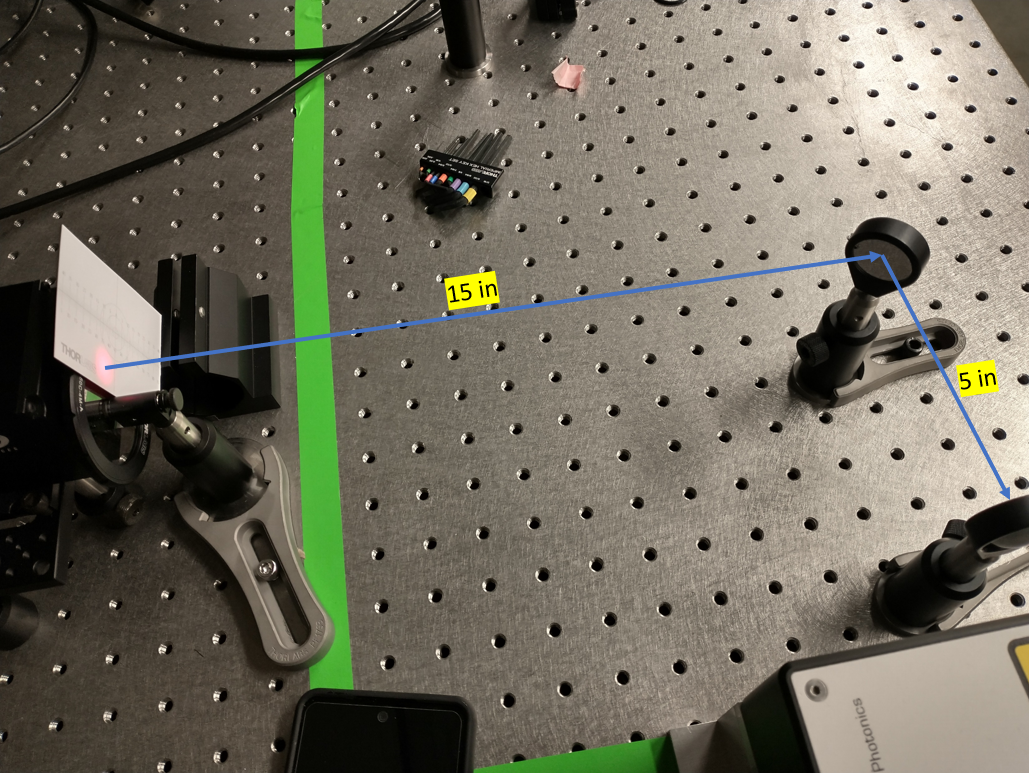
\includegraphics[width=\textwidth]{figures/distance_drawing.png}
         \caption{Approx. bounce path measurement}
         \label{fig:light_path_measured}
     \end{subfigure}
        \caption{Bounce Path Analysis}
        \label{fig:light_path_all}
\end{figure}

Using the approximate measurements from the pictures of the setup, we get a traversal time from the ND filter back to the 45 degree mirror of 2.54ns (the most likely bounce path upon inspection of the light reflecting off the sides).

\[
\Delta T=15\ in * 2 * \frac{2.54\ cm}{1\ in} * \frac{1\ m}{100\ cm} * \frac{1}{c} = 2.54 ns
\]

While this is on a similar scale to the FWHM measured as 100ps, it is too large to have caused a spreading from 5ps to 100ps, as that would mean a point spread function with temporal width of 95ps. 

Although it appears this is not the cause of the disparity in pulse width measurements, another (and much shorter) bounce path could be between the aperture of the photon counter and the ND filter, though the likelihood is much lower due to better attenuation from the surface of the photon counter. The distance in this case is approximately 0.5", which yields via the previous equation a bounce time from aperture to ND filter and back of 85ps, which is much closer to the 95 ps expected for the bounce time. However, due to that being the only possible bounce path, and having no shorter ones available , the expected pulse as a result of that would be a convolution of the input pulse and 2 impulses, one at t=0ps, and another at t=85ps (or whatever the true bounce time is). This would merely duplicate the pulse at each impulse, rather than spreading out the pulse over the entirety of the time segment from t=0 to t=85ps.

For the above reasons, it appears that the bounce analysis does not conclusively account for the spreading of the laser pulse, although it may be affecting the pulse shape to a lesser degree. Other sources of error into the system must be analyzed to properly account for the source of this dispersion.

\section{Literature Review}
\subsection{Photon Counting Paper AO1984}

This paper discusses a computational method of signal reconstruction and phase recovery using the Fourier transform of the triple-correlation of a signal, the bi-spectra. The bi-spectra is important as it may be gained via a Hanbury-Brown-Twiss interferometer setup, which then can be fed through this algorithm to gain the original signal.

The triple correlation of a signal is simply an extension of the familiar correlation function into 2 dimensions.

\[ 
R_{fff}\left(\tau_1,\tau_2\right)=\int_{-\infty}^{\infty}f\left(t\right)f\left(t+\tau_1\right)f\left(t+\tau_2\right)dt
\]
The result of this is a 2D function, with the shifts as the parameters. An easy way to visualize this is to plot the 3 versions of f(t) above each other, and then plot the multiplication of the three below those. The integral of that bottom function is the value of the triple-correlation at that $\tau_1$,$\tau_2$. 

\begin{figure}
\centering
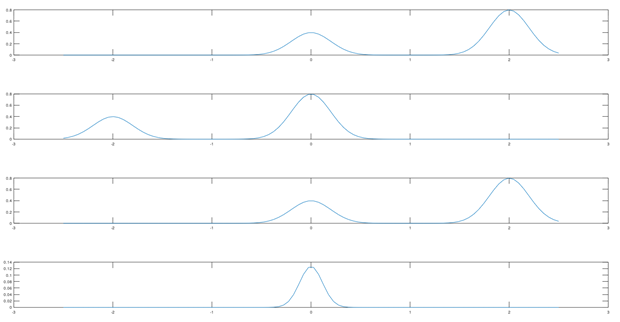
\includegraphics[width=1.0\textwidth]{figures/triple_correlation.png}
\caption{\label{fig:triple_correlation_explanation}Triple correlation pieced together.}
\end{figure}

\begin{figure}
\centering
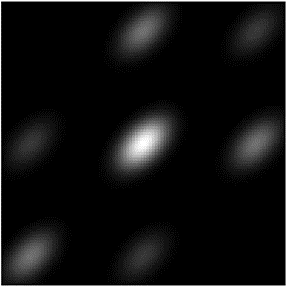
\includegraphics[width=0.8\textwidth]{figures/triple_correlation_img.png}
\caption{\label{fig:triple_correlation_img}Triple correlation 2D function evaluation.}
\end{figure}
With the bispectra being an available measurement from which to attempt to recover the original signal,  it is useful to notice that the bispectra is essentially the fourier transform of the original signal multiplied by itself with different shifts:

\[T\left(x_1,x_2\right)=  \int T\left(x\right)T\left(x+x_1\right)T(x+x_2)\]
\[\mathcal{F}\left(T\left(x_1,x_2\right)\right)\left(w_1,w_2\right)=\ \widetilde{T}(w_1)\widetilde{T}(w_2)\widetilde{T}(-w_1-w_2)\]
Where $\widetilde{T}(w)$ is the Fourier transform of the original signal. The paper then proves their assertion that \textit{If T(x) is real and of finite extent, T(x) can be reconstructed from its bispectrum except for a shift a. Equivalently, the Fourier transform T(u) of T(x) is determined except for a linear phase factor.}

They begin with the proof that the bispectrum is unaffected by a time shift in T, or a multiplication by a linear phase shift in the frequency domain (which are equivalent operations).

\section{Conclusion \& Future work}

\bibliographystyle{alpha}
\bibliography{sample}

\appendix
\newpage
\section{Deconvolution MATLAB/OCTAVE script}
\verbatiminput{deconvolution.m}
\section{Data processing and FWHM calculation Python script}
\verbatiminput{full_width_half_max.py}
\section{Triple correlation example MATLAB/OCTAVE script}
\verbatiminput{full_width_half_max.py}

\end{document}